\documentclass[]{beamer}
% Class options include: notes, notesonly, handout, trans,
%                        hidesubsections, shadesubsections,
%                        inrow, blue, red, grey, brown

% Theme for beamer presentation.
\usepackage{beamerthemesplit} 
% Other themes include: beamerthemebars, beamerthemelined, 
%                       beamerthemetree, beamerthemetreebars  

\title{PHY115}    % Enter your title between curly braces
\author{Free Falling Motion}                 % Enter your name between curly braces
\institute{Digipen}      % Enter your institute name between curly braces
\date{Spring 2023} 

\begin{document}

% Creates title page of slide show using above information
\begin{frame}
  \titlepage
\end{frame}
%\note{Talk for 30 minutes} % Add notes to yourself that will be displayed when
                           % typeset with the notes or notesonly class options

\section[]{}

% Creates table of contents slide incorporating
% all \section and \subsection commands
\begin{frame}
  \tableofcontents
\end{frame}

%%%%%%%%%%%%%%%%%%%%%%%%%%%%%%%%%%%%%%%%%%%%%%%%%%%%%%%%%%%%%%%%%%%
\section{Free fall}
\subsection{Free falling bodies}

%%%%%%%%%%%%%%%%%%%%%%%%%%%%%%%%%%%%%%%%%%%%%%%%%%%%%%%%%%%%%%%%%%%
\begin{frame}
    Free fall:
    \vspace{3mm}

\begin{enumerate}
\item Between  1589 and 1592 $\rightarrow$ Galileo's experiment:
      \begin{itemize}
          \item He dropped two spheres of different masses from the Tower 
          of Pisa and  demonstrated that their falling time was independent of their mass
      \end{itemize}
      \pause
      \vspace{3mm}

\item In 1687 $\rightarrow$ Newton's Laws
    \begin{itemize}
        \item He published \textit{"Philosophiæ naturalis principia mathematica"}, the laws that describe this experiment.
    \end{itemize}

\end{enumerate}
 
\vspace{3mm}

    Video: \url{https://www.youtube.com/watch?v=QyeF-_QPSbk}

\end{frame}  

%%%%%%%%%%%%%%%%%%%%%%%%%%%%%%%%%%%%%%%%%%%%%%%%%%%%%%%%%%%%%%%%%%%
\begin{frame}
    Free fall:
    \vspace{3mm}
Newton's Law:
\vspace{3mm}


  \begin{columns}[c]
    \column{2in}  % slides are 3in high by 5in wide
   
    The magnitude of the acceleration that the Earth makes on a body is:
    \begin{equation*}
        g=G\frac{M}{d^2}
    \end{equation*}
    
    $d$ is the distance between the body and the center of the Earth.
    \vspace{2mm}

    \begin{itemize}
        \item $G= 6,67·10^{-11} $ Nm$^{2}$/kg$^{2}$
        \pause

        \item $M=5,972 \times 10^{24}$ kg
    \end{itemize}
    
 
    \column{2.5in}
    
    \begin{figure}[h!]  
        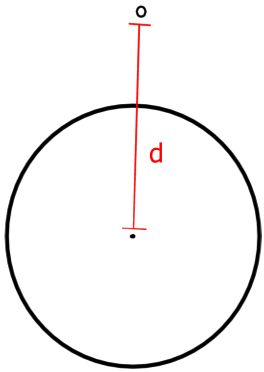
\includegraphics[width=0.6\textwidth]{images/5.jpg}
       
      \end{figure}
 
 
 
    \end{columns}

\end{frame}  

%%%%%%%%%%%%%%%%%%%%%%%%%%%%%%%%%%%%%%%%%%%%%%%%%%%%%%%%%%%%%%%%%%%


\begin{frame}
   What happens when the bodies near the Earth surface? 
    \pause
    
    \vspace{3mm}

        \begin{equation*}
            g=\frac{GM}{(h+R)^2}=\frac{GM}{\big[R(\underbrace{\frac{h}{R}}_{\approx 0}+1)\big]^2}
        \end{equation*}

        \begin{equation*}
         \rightarrow   g\approx\frac{GM}{R}\approx9.8~m/s^2
        \end{equation*}

        \begin{figure}[h!]  
            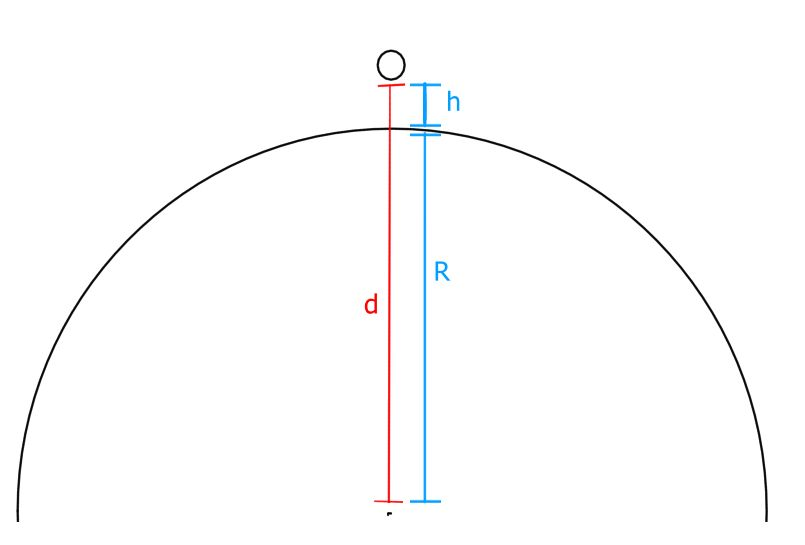
\includegraphics[width=0.6\textwidth]{images/6.jpg}
            
          \end{figure}
     
    \end{frame}

%%%%%%%%%%%%%%%%%%%%%%%%%%%%%%%%%%%%%%%%%%%%%%%%%%%%%%%%%%%%%%%%%%%

\begin{frame}
    Free fall:
    \vspace{3mm}
\begin{itemize}
\item  Body falling under the influence of the earth’s gravitational attraction.
\pause
\item  If the effects of the air can be neglected, all bodies fall with the 
same downward acceleration, regardless of their size or weight.
\pause 
\item If  the fall is small compared with the radius of the earth, and if we ignore small effects due to the
earth’s rotation, the acceleration is constant.
\end{itemize}
 
    

\end{frame}

%%%%%%%%%%%%%%%%%%%%%%%%%%%%%%%%%%%%%%%%%%%%%%%%%%%%%%%%%%%%%%%%%%%


\begin{frame}
    The constant acceleration of a freely falling body is called the \textbf{acceleration
    due to gravity}, and we denote its magnitude with the letter $g$.
    \vspace{3mm}
    
    Near the surface of the earth.
    \pause

    \begin{equation}
    g=9.8~m/s^ 2
    \end{equation}
    
    \pause

  

    Near the surface of the moon:
    \pause
    \begin{equation}
        g=1.6~m/s^ 2
        \end{equation}
        
        \pause

  

        Near the surface of the sun:
        \pause
        \begin{equation}
            g=270~m/s^ 2
            \end{equation}
    
      
    
     % \begin{center}
     % 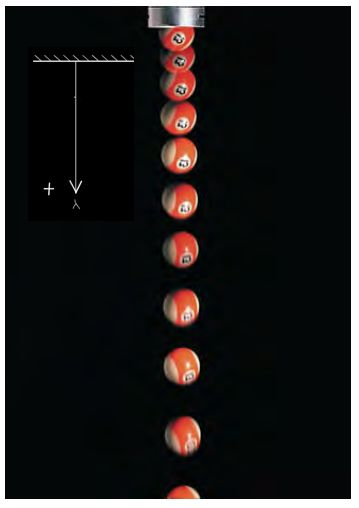
\includegraphics[height=1.in]{images/2.jpg}
    %\end{center}
     \end{frame}

%%%%%%%%%%%%%%%%%%%%%%%%%%%%%%%%%%%%%%%%%%%%%%%%%%%%%%%%%%%%%%%%%%%




\begin{frame}
   \textbf{g is always a positive number}  
   \vspace{3mm}


   Because g is the magnitude of a vector quantity,
    it is always a positive number.
     \end{frame}

%%%%%%%%%%%%%%%%%%%%%%%%%%%%%%%%%%%%%%%%%%%%%%%%%%%%%%%%%%%%%%%%%%%


\begin{frame}
EXAMPLE 3.1


\vspace{3mm}

 \begin{columns}[c]
    \column{2in}  % slides are 3in high by 5in wide
   
    \begin{equation}
       x(t)=-\frac{1}{2}gt^ 2+v_0t+x_0
        \end{equation}
 
 
    \column{2.5in}
    
    \begin{figure}[h!]  
   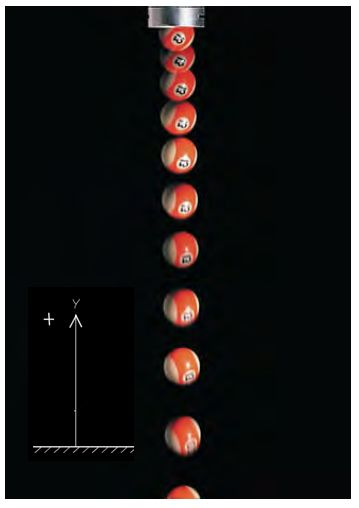
\includegraphics[width=0.8\textwidth]{images/1.jpg}
    \caption{Position vs. time. {\tiny Figure from Sears and Zemansky's University Physics 
    with Modern Physics, 13th Edition.} }
 \end{figure}
 
 
 
    \end{columns}
 
\end{frame}


%%%%%%%%%%%%%%%%%%%%%%%%%%%%%%%%%%%%%%%%%%%%%%%%%%%%%%%%%%%%%%%%%%%


\begin{frame}
    EXAMPLE 3.2
    
    \vspace{3mm}
    
     \begin{columns}[c]
        \column{2in}  % slides are 3in high by 5in wide
       
        \begin{equation}
           x(t)=\frac{1}{2}gt^ 2+v_0t+x_0
            \end{equation}
     
     
        \column{2.5in}
        
        \begin{figure}[h!]  
       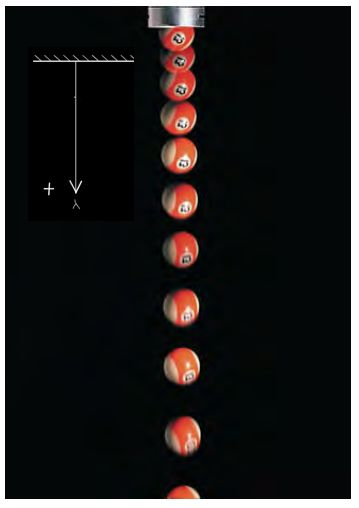
\includegraphics[width=0.8\textwidth]{images/2.jpg}
        \caption{Position vs. time. {\tiny Figure from Sears and Zemansky's University Physics 
        with Modern Physics, 13th Edition.} }
     \end{figure}
     
     
     
        \end{columns}
     
    \end{frame}


%%%%%%%%%%%%%%%%%%%%%%%%%%%%%%%%%%%%%%%%%%%%%%%%%%%%%%%%%%%%%%%%%%%


\begin{frame}
    EXERCISE 3.1
    \pause
    
    \vspace{3mm}

    A one-euro coin is dropped from the Leaning Tower of Pisa and
    falls freely from rest. What are its position and velocity after 1.0 s,
    2.0 s, and 3.0 s?
     
    \end{frame}




%%%%%%%%%%%%%%%%%%%%%%%%%%%%%%%%%%%%%%%%%%%%%%%%%%%%%%%%%%%%%%%%%%%


\begin{frame}
    EXERCISE 3.2
  
    You throw a ball vertically upward from the roof of a building.
        The ball leaves your hand with
        an upward speed of $15~m/s$; the ball is then in free fall. Find 
        \pause
    \vspace{3mm}

    \begin{enumerate}
        \item the ball’s position and velocity $1.00~s$ and $4.00~s$ after leaving your hand;
        \pause
        \item the ball’s velocity when it is $5.00~m$ above the railing;
        \pause
        \item the maximum height reached;
        \pause
        \item the ball’s acceleration when it is at its maximum height.
    \end{enumerate}
    
    \end{frame}



%%%%%%%%%%%%%%%%%%%%%%%%%%%%%%%%%%%%%%%%%%%%%%%%%%%%%%%%%%%%%%%%%%%


\begin{frame}
    EXERCISE 3.2
  
    \begin{center}

        \begin{figure}[h!]  
            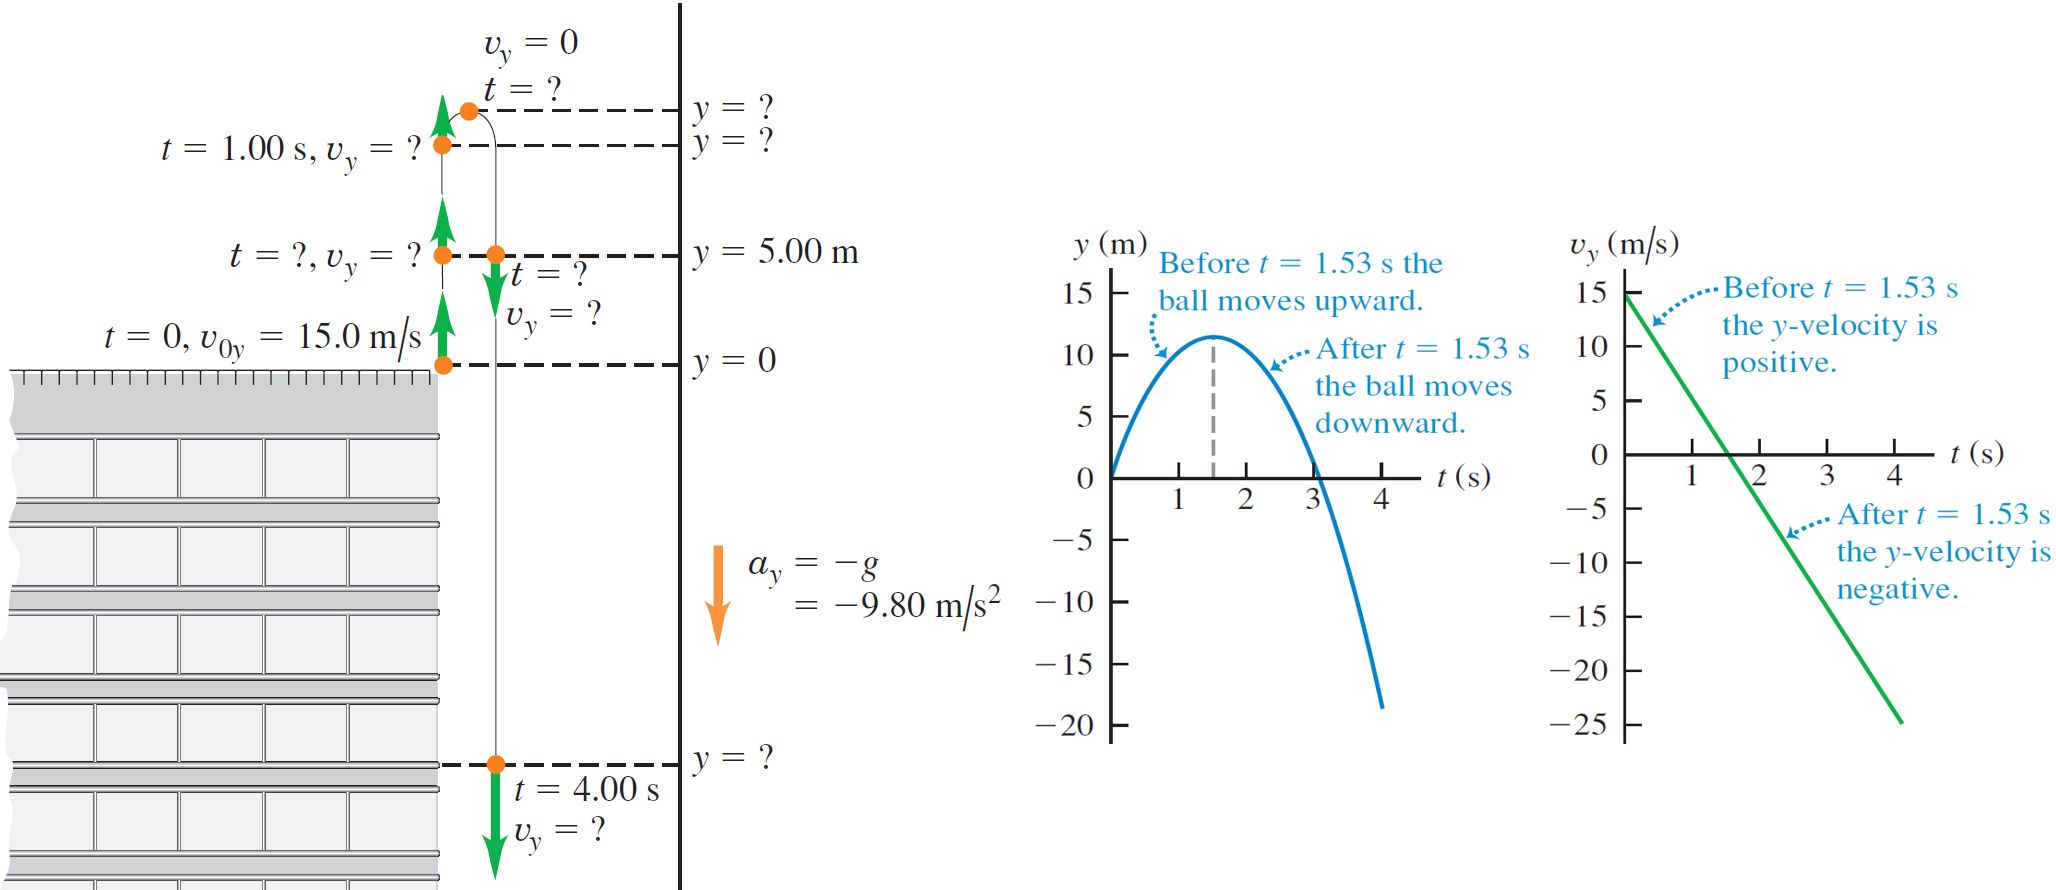
\includegraphics[width=1.1\textwidth]{images/3.jpg}
             \caption {{\tiny Figure from Sears and Zemansky's University Physics 
             with Modern Physics, 13th Edition.} }
          \end{figure}
        
    \end{center}

      
    
    \end{frame}






%%%%%%%%%%%%%%%%%%%%%%%%%%%%%%%%%%%%%%%%%%%%%%%%%%%%%%%%%%%%%%%%%%%


\begin{frame}
    Test Your Understanding
    \vspace{3mm}
    \pause

If you toss a ball upward with a certain initial speed, it falls freely and reaches a maximum 
height h a time t after it leaves your hand.
\vspace{3mm}

\pause
\begin{itemize}
    \item If you throw the ball upward with double the initial speed,
    what new maximum height does the ball reach?
    \pause
        \begin{enumerate}
            \item $h\sqrt{2}$
            \item $2h$
            \item $4h$
            \item $8h$
            \item $16h$
        \end{enumerate}

\end{itemize}

    
    \end{frame}

%%%%%%%%%%%%%%%%%%%%%%%%%%%%%%%%%%%%%%%%%%%%%%%%%%%%%%%%%%%%%%%%%%%


\begin{frame}
    Test Your Understanding
    \vspace{3mm}
 
    
If you toss a ball upward with a certain initial speed, it falls freely and reaches a maximum 
height h a time t after it leaves your hand.
\vspace{3mm}


\begin{itemize}
        \pause
    \item If you throw the ball upward with double the initial speed, how long does it take to
    reach its new maximum height?
        \begin{enumerate}
            \item $t/2$
            \item $t/\sqrt{2}$
            \item $t$
            \item $t\sqrt{2}$
            \item $2t$
        \end{enumerate}
\end{itemize}

    
    \end{frame}



%%%%%%%%%%%%%%%%%%%%%%%%%%%%%%%%%%%%%%%%%%%%%%%%%%%%%%%%%%%%%%%%%%%
 \end{document}
%%%%%%%%%%%%%%%%%%%%%%%%%%%%%%%%%%%%%%%%%%%%%%%%%%%%%%%%%%%%%%%%%%%